\documentclass[10pt, compress, xcolor={usenames,dvipsnames}]{beamer}


%%% Theme and style
\usetheme{metropolis}
\metroset{progressbar=frametitle}
\metroset{numbering=fraction}

%%% Packages %%%

% Use T1 and a modern font family for better support of accents, etc.
\usepackage[T1]{fontenc}
\usepackage{palatino}  % Palatino
% \usepackage{lmodern}

% Language support
\usepackage[english]{babel}

% Support for easily changing the enumerator in
% enumerate-environments.
\usepackage{enumerate}

% Support for importing images
%\usepackage{graphicx}

% Use hyperlinks
\usepackage{hyperref}

% Don't load xcolors package in beamer: use document class option
% instead...
%\usepackage[usenames,dvipsnames]{xcolor}

% Use colors in tables
%\usepackage[pdftex]{colortbl}

% A nice monospace font for listings, etc.
%\usepackage[scaled]{beramono}
%\usepackage{inconsolata}
\setmonofont{DejaVu Sans Mono}

% Using TikZ for diagrams
\usepackage{tikz}
\usetikzlibrary{shapes,mindmap}
%\usetikzlibrary{er,mindmap,calc,intersections,shapes,arrows,fit,matrix,positioning,decorations.pathmorphing,topaths,trees,automata}
\usepackage{tikz-cd} % for CM-arrow tips.

% Don't use externalize with gradients!!!
%\usetikzlibrary{external,arrows,fit,matrix,positioning}
%\tikzexternalize % Activate externalizing TikZ graphics.

\usepackage{pifont} % for ding
\usepackage[inline]{enumitem}
\usepackage{xspace}
\usepackage{listings}
\usepackage{minted}

% Scala listings.  Use colored Scala style by default.
\usepackage{lstscala}
\lstnewenvironment{lstscalasmall}{%
  \lstset{style=scala-color,basicstyle=\scriptsize\tt}}{}

\colorlet{ImportantCode}{ForestGreen}
\colorlet{ImportantCode2}{RubineRed}

\lstset{style=scala-color}

\lstnewenvironment{Scala}
  {\lstset{
    style=scala-color,
    flexiblecolumns=false,
    mathescape=false,
    basicstyle=\small\color{blue!30!darkgray}\tt}}
  {}


%%%% Custom macros %%%%
\newif\ifcompileTreeSlides
%\compileTreeSlidesfalse
\compileTreeSlidestrue

\newcommand{\SmallArrow}{\ding{228}}
\newcommand{\BigArrow}{$\longrightarrow$\xspace}
\newcommand{\Triangle}{$\triangleright$\xspace}
\renewcommand{\emph}[1]{\alert{#1}}
\newcommand{\light}{\color{TealBlue}}
\renewcommand{\hbar}{{\color{mLightBrown}\hrulefill}}

% http://tex.stackexchange.com/a/56585/77356
\tikzset{
  invisible/.style={opacity=0},
  visible on/.style={alt=#1{}{invisible}},
  alt/.code args={<#1>#2#3}{%
    \alt<#1>{\pgfkeysalso{#2}}{\pgfkeysalso{#3}} % \pgfkeysalso doesn't change the path
  },
}

%%% Document info %%%

\title{An implementation of SGP4  \\
in non-singular variables  \\
using a functional paradigm}

\author{Pablo Pita Leira}

% To show the TOC at the beginning of each section, uncomment this:
% \AtBeginSection[]
% {
%   \begin{frame}<beamer>{Outline}
%     \tableofcontents[currentsection]
%   \end{frame}
% }

% To show the TOC at the beginning of each subsection, uncomment this:
% \AtBeginSubsection[]
% {
%   \begin{frame}<beamer>{Outline}
%     \tableofcontents[currentsection,currentsubsection]
%   \end{frame}
% }


% To uncover everything in a step-wise fashion, uncomment this:
% \beamerdefaultoverlayspecification{<+->}


\date{%
  \small 15th March 2016\\[2em]
  6\textsuperscript{th} ICATT Conference, Darmstadt}
%  \includegraphics[height=7mm]{img/epfl-logo}}


%%% Start of the actual document %%%

\begin{document}

\begin{frame}
  \titlepage
\end{frame}

% No outline, too short a talk...
% \begin{frame}{Outline}
%   \tableofcontents
%   % You might wish to add the option [pausesections]
% \end{frame}

\section{Motivation}

\begin{frame}[fragile]{SGP4}
Simplified General Perturbations 4 orbit propagator

\begin{itemize}[label=\SmallArrow]
\item  widely used tool for the fast, short term propagation of earth satellite orbits
\item  thoroughly described in the SPACETRACK report \#3 by Hoots et al.
\item  numerous versions of SGP4: FORTRAN, C++, Java, MATLAB
\item  Inputs: two line elements (TLE) disseminated by NORAD
\end{itemize}

%  \vspace{1em}

\end{frame}

\begin{frame}[fragile]{SGP4 Algorithm Description}

\begin{itemize}[label=\SmallArrow]
\item applied for all orbits with periods of T <= 225 min.
\item secular rates of change due to the zonal harmonics J2 and J4 of the Earth potential,
 and due to drag perturbations in an atmosphere with a power-law altitude profile of air density
\item long period corrections perturbations due to J3
\item first-order, short-period perturbation corrections due to J2
\end{itemize}

%  \vspace{1em}

\end{frame}


\begin{frame}[fragile]{SGP4Extensions: why one more version?}

SGP4 is used in a broader context like conjunction analysis.

Scala can be interesting for the design of algorithms in this broader context

By having a version of SGP4 in Scala, the integration of SGP4 in the algorithms is easier.

SGP4Extensions exposes new function calls that enables new conjunction algorithms

No implementation of SDP4

\end{frame}

\section{SGP4Extensions}

\begin{frame}[fragile]{Scala}

Developed by Martin Odersky in the EPFL since 2001.

  \begin{itemize}[label=\SmallArrow]
    \item Hybrid object oriented/functional
    \item Rich type system
    \item compiled to java byte code, also possible javascript
    \item designed for creating DSL on top: expressive
  \end{itemize}

\end{frame}

\begin{frame}[fragile]{SGP4Extensions: characteristics}

  \begin{itemize}[label=\SmallArrow]
  \item  It is heavily influenced by the functional software paradigm.
  \item  Equations have been expressed almost always literally writing the algebraic equations in the code as expressed in the papers
  \item  Implementations using other variables and/or extra terms can be easily introduced into the propagation algorithm
  \item  Provides more options and flexibility when being used within other algorithms, like those performing space debris conjunction analysis

  \end{itemize}

\end{frame}

\begin{frame}[fragile]{Unicode support}

  \begin{itemize}[label=\SmallArrow]
    \item Unicode support to express equations
	\item Lyddane 2nd Order Long Period Corrections:
  \end{itemize}

  %\begin{minted}{scala}
%  \begin{Scala}

val $\delta I =  \epsilon 3*e\sin\omega * c$

val $\delta a =  0$

val $\delta h = -\epsilon 3*e\cos\omega* c/s$

val $\delta C = -\epsilon 3*e\cos\omega* e\sin\omega * (1/s - 2*s)$

val $\delta S =  \epsilon 3*s - \epsilon 3*`\eta^2`*s - 2*\epsilon 3*`e\cos\omega ^2`*s + \epsilon 3*`e\cos\omega ^2`/s$

val $\delta F =  \epsilon 3*s* e\cos\omega * (1 - 2*`\eta^2`/(1+\eta)) / 2$

Note: $e\cos\omega ^2$ that the product $e\cos\omega$ is squared.

%\end{Scala}
%\end{minted}

\end{frame}


\begin{frame}[fragile]{SGP4 Vallado model}
  \begin{figure}
    \centering
    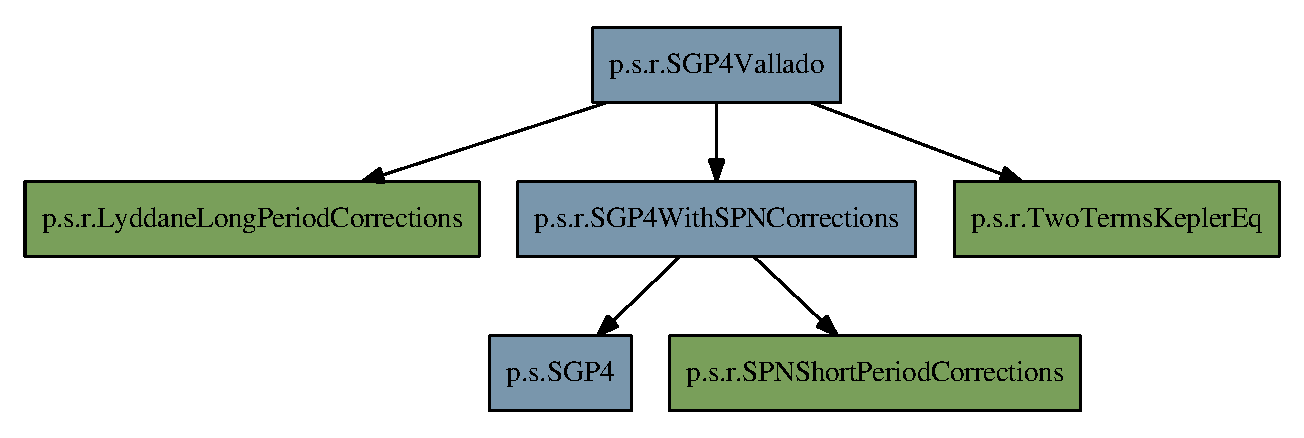
\includegraphics[width = 1.0\textwidth]{vallado}
  \end{figure}
\end{frame}

\begin{frame}[fragile]{SGP4 Lara model}
  \begin{figure}
    \centering
    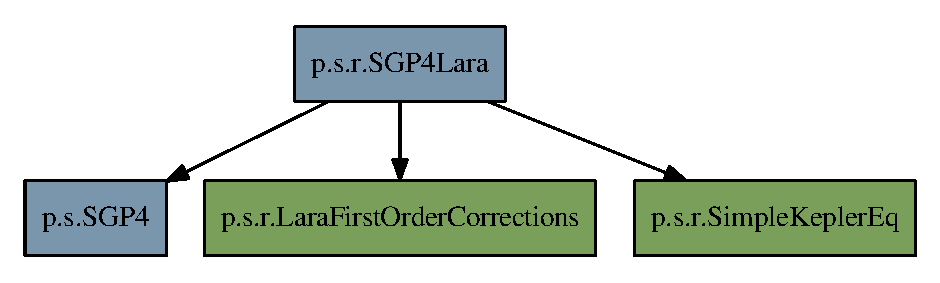
\includegraphics[width = 1.0\textwidth]{lara}
  \end{figure}
\end{frame}

\begin{frame}[fragile]{Validation results}
Tested with TLEs for near Earth used by David Vallado
  \begin{itemize}[label=\SmallArrow]
    \item SGP4Vallado match C++ results (max diffs $10^{-8}$) at 30000 min
    \item Order of calculation of Kepler equation does not introduce significant effects
    \item There are small differences between other algorithms like PolarNodals, Lara and ValladoLong with SGP4Vallado
  \end{itemize}
\end{frame}

\section{What's next}

\begin{frame}[fragile]{Future's work}
  \begin{itemize}[label=\SmallArrow]
    \item Propagation of the whole catalog
    \item Collision analysis
    \item Conjuctions in field of view of optical cameras
  \end{itemize}
\end{frame}

\plain{\Huge Questions?}

\end{document}

% vim: spell spelllang=en_gb
% vim: set tabstop=2 softtabstop=2 shiftwidth=2 textwidth=80: %
